This dissertation represents the culmination of my nearly seven years at Stanford, and I've been thinking about writing this section for the last three. And yet, sitting here at my desk at the University of Colorado, I find myself at a lack for words.

Finishing this dissertation feels oddly anticlimactic. Going into a Ph.D program, one tends to believe a dissertation is the result of focused, thoughtful research on a long, but straightforward path. But my path was by no means direct, and after all of it, I'm left with more questions than answers.

I joined the VLF group at Stanford, a bustling research conglomerate of roughly twenty students, a half dozen research scientists, and two staff engineers, in October 2011. Less than two years later, I found myself, along with fellow student Chris Young, dragging four heavy Pelican cases through rush-hour crowds at a train station in Kagoshima, Japan, as part of a whirlwind ten-day stint installing three VLF radio receivers in Sapporo, Kagoshima, and Mt. Fuji. At the same time, I had been entrusted, along with a handful of other students, with designing a CubeSat -- which would go to \emph{space!} -- a project which at the time felt both incredible and overwhelming. The excitement within the group was palpable, fueled by a driven professor and supported by the well-trained machinery of the senior research staff.

Unfortunately, following the semi-retirement of our professor Dr. Umran Inan and the department's disinterest in hiring a replacement, our ranks began to dwindle. Other groups brought in new students and new projects, but I was one of a final few. The excitement dwindled; the research meetings grew smaller and smaller. Labs were shut down, equipment surplussed, and the open doors of professors remained frequently shut. The once-bustling basement of the Packard building felt like a ghost town, with dust collecting on the remnants of a brighter age.

Over the following months I gradually transitioned to the SESS lab, directed by Dr. Sigrid Close, in the Aeronautics / Astronautics department, along with then research scientist Dr. Robert Marshall. Joining the SESS lab, and being immersed in a new variety of wide-reaching research topics rekindled some of that lost excitement. Not soon thereafter, however, Dr. Robert Marshall secured a coveted faculty position at CU Boulder. I found myself again pursuing a project in isolation from other students, and once again without an in-person mentor.

Saying that a Ph.D is ``hard'' is a simplification. In my experience, the papers and the math are understandable. The courses, despite occupying a substantial portion of one's time, are doable. But a Ph.D is a mind game: Learning to explore an unknown topic without guidance, and to focus without a destination in mind, all while trying to take classes, pay rent, and thrive amidst the meritocratic culture and soaring wealth inequality of Silicon Valley was no easy task. And it was only through bullheaded, stubborn foolishness that I persisted.

I defended my research in July 2017. Afterward, Dr. Marshall offered me an early postdoctoral position in his lab at the University of Colorado Boulder, which could overlap with the completion of my dissertation. I accepted and moved to Boulder in October, 2017. Colorado was the breath of fresh mountain air I desperately needed: The bulk of this dissertation was written here at CU.

I'm immensely proud of the work presented here, and am pleasantly surprised to see a coherent thread stitch together the various projects I've worked on. In some sense, I did the research entirely backwards: beginning first with instrument design (as in chapter \ref{chapter:VPM}), then investigating an existing model, then finally diving headfirst into the minute details to emerge with the improved numeric simulations presented in chapters \ref{chapter:power} and \ref{chapter:global_estimates}.

And yet, despite presenting a complete model with some interesting results, I find myself with more questions than answers. What have we overlooked? Where could we improve? And how could our results, which are broad in space and time, be conclusively measured?
\\
\indent I suppose this is how academics are born.
%
%Going into a Ph.D program, you tend to think of a dissertation as a final, be-all, end-all answer, a pinnacle of unrelenting, focused, thoughtful research, culminating in The Great Answer to your questions. Now, at the end of my program, however, this dissertation feels oddly anticlimactic. My path to this point was by no means direct: graduate research is by nature a meander, a random walk trajectory through courses and projects and countless research papers. There's no straight line to the finish - but there is, with enough guidance, a drift. 
%
%By no means would I say I've arrived at the fabled ``answer''. I don't feel a sense of enlightenment. My work here has left me with an ever-expanding set of questions, model improvements, approximations and assumptions in need of scrutiny. But in a sense that is the destination for the countless hopeful academics who have embarked on a Ph.D. At the end, there are only more questions.
%
%My particular path through Stanford was not direct at all. I entered as a first year student in the VLF group, which focused on low-frequency radio waves in the magnetosphere. The VLF group was built on over 50 years of geophysics and radioscience research at Stanford, and consisted of a thriving collection of a half-dozen research staff and nearly twenty graduate students, under the direction of Dr. Umran Inan. I knew early on that the VLF group had reached the end of its lifespan going into it, but had been assured that things would continue smoothly, that there would be people to work with, and that I would be one of a handful of final students to carry the VLF banner.
%
%Within my first couple years, I worked on several interesting and unique research opportunities -- beginning first with hardware design for a CubeSat (see chapter \ref{chapter:vpm}),
%
%VLF waves traverse great distances, and research on these waves follows accordingly. The VLF group prided itself on maintaining a global network of student-maintained radio receivers, from Alaska to Antarctica. Less than two years in as a student, I found myself, along with fellow student Chris Young, dragging four heavy Pelican cases through the rush-hour crush of a train station in Kagoshima, Japan, as part of a whirlwind ten-day stint installing three such receivers in Sapporo, Kagoshima, and Mt. Fuji. Similarly, I had been entrusted, along with a handful of other students, with designing a CubeSat -- which would go to space! -- which at the time felt both incredible and overwhelming. The excitement within the group was palpable, fueled by a driven professor and supported by the well-trained machinery of the senior research staff.
%
%Unfortunately, things were somewhat built to spill, and as the quarters progressed steadily on, our ranks began to dwindle. Other groups brought in new students and new projects; but I was the last one in the door. The excitement dwindled; the research meetings grew smaller and smaller. Labs were shut down, equipment surplussed, and the open doors of professors remained frequently shut. The once-bustling basement of the Packard building felt like a ghost town, with dust collecting on the remnants of a brighter age.
%
%As the group continued to shrink, my research advisor, Dr. Sigrid Close, graciously took me into her lab in the Aerospace Engineering department, along with VLF research scientists Dr. Robert Marshall and Dr. Ivan Linscott. Switching to the AA department was a fantastic opportunity to escape the loneliness and gloom of the Packard basement lab. Courses and research continued on, now in an active research group (and with daylight windows!). Not soon thereafter, however, Dr. Robert Marshall secured a coveted faculty position at CU Boulder. I found myself again pursuing a project in isolation from my fellow students, and once again without an in-person mentor.
%
%The fourth year was the by far the hardest. Four years was too far in to quit, and yet the end was nowhere in sight. My research was unfocused and unguided; my funding was swiftly running out, and the financial realities of trying to pay rent in silicon valley amidst rampant inequality and a perpetual housing shortage left me feeling overwhelmed and uninspired. 
%
%Shortly thereafter I moved further away from campus, into a shared house with some friends. I made a conscious effort to nourish my life outside of the Stanford bubble. Through perseverance and dedication, and with the guidance of Dr. Close and, remotely, with Dr. Marshall, I succeeded at developing the work presented in this dissertation and defended in July, 2017.
%
%Dr. Marshall offered me an early postdoctoral position in his lab at the University of Colorado Boulder, which could overlap with the completion of my dissertation. I accepted and moved to Boulder in October, 2017. Boulder was the breath of fresh mountain air I desperately needed. The bulk of this dissertation was written here at CU.
%

There are countless people who, without their invaluable guidance, I would not be writing this section today. First and foremost, to my mentor, Dr. Robert Marshall, who has been perhaps the one constant thread throughout my seven years: first as a faculty mentor on the VPM project, then as a co-advisor in the AA department, and now as my PI at the University of Colorado. Bob, you're an inspiration.

To my advisor, Dr. Sigrid Close, who took me in despite having an already overwhelming cadre of students. Dr. Close strives to cultivate creativity, and would let brainstorming sessions run rampant. I've always appreciated our conversations, and that you'd let them meander to topics far beyond the research at hand.

To Dr. Antony Fraser-Smith, who as graciously served as my third committee member, especially while recovering from a heart surgery. Tony has been an integral part of the radioscience community at Stanford since 1968, and is a wellspring of interesting stories, entertaining anecdotes, and exudes the good-natured, jovial personality that makes geoscience a compelling world to work in. Furthermore, Dr. Fraser-Smith was responsible for putting together the Villard Fellowship for Students in Radioscience, in memory of the late Dr. Oswald Garrison Villard Jr., which supported my first year of research, and was the deciding factor in my attending Stanford. 

To the researchers and engineers who kept the VLF group running, and continued to offer assistance well beyond their obligations: Dr. Ivan Linscott, Dr. Dave Lauben, and Dr. Morris Cohen, who made themselves available for any and every question I had, no matter how trivial. A special thank you to Dr. Maria Spasojevic, who took the time to personally call me when I was applying to grad school.
 
To Jeff Chang, who singlehandedly ran every technical aspect of the VLF group, from the compute cluster to PCB layout to metal manufacturing.
 
To Professor Emiko Yasumoto, who showed special concern for my well-being during a particularly rough time in my fourth year. \begin{CJK}{UTF8}{min}ありがとうございます!\end{CJK}

To Dr. Forrest Foust, a former VLF'er and the author of the ray tracing code used within this dissertation. Despite having left for the greener pastures of industry, Forrest eagerly and wholeheartedly jumped in to diagnose and fix some erroneous results I could not understand.

Naturally, to my parents, both of whom have made their careers in biology and wildlife sciences, who nurtured an interest in thinking creatively, and instilled in me a lifelong appreciation for learning -- despite what my 18-year-old self may have said. Having grown up in Alaska, under the pale winter glow of the northern lights, it's no surprise that I should end up writing a dissertation on space science.

To my friends, colleagues, and lunch buddies from the VLF and SESS groups: Chris Young, with whom I've shared adventures across Japan, and the best magician I know; David Freese, for dragging me up Half Dome in the middle of the night; Patrick Blaes, for teaching me everything I know about research computing. To Rasoul Kabirzadeh, for enduring the same struggles along with me. To Sid, Nicholas, Anna, Lorenzo, and everyone in the SESS group who welcomed me in halfway through my program: Thank you all.

I owe a truly incalculable debt of gratitude to my community outside of campus, who without their constant companionship I most surely would have turned tail and returned to Seattle in 2012. To Ted Phares, for 2 AM snacks and 2 PM breakfast. To Tristan Hudson, an amazingly talented engineer who speaks three languages, shreds on the piano, and can quote a rap lyric about any topic whatsoever. To Damien Heiser and Wayne Tsai, for bringing me to Burning Man -- twice (so far). To Galen, Abe, JDT, Mike, Phil, Dan, Ricky, Hukka, Max, and everyone else: more than the classes, more than the research: you guys made me the person I am today, and I would not be here without you. Thank you.

To Bob Lang and Stuart Hallerman, for inspiring me to study electronics in the first place.

To my partner of nearly 9 years, Ty Logan: Thanks for listening to me ramble about lightning all day and night.

Finally, to my high school history teacher, Mark Rippy: In my senior year, I was assigned to write a history paper and I flat-out refused to do it. Mark brushed it off with the following simple advice: ``Nobody else will do it for you." It was a bombshell, and it changed my life. It sounds silly, but those words became a mantra that got me through high school, an Associate's degree, five years in the music industry, two Bachelor's degrees, a Master's degree, and now, a Stanford doctorate. Teachers change lives in tremendous ways, every day, even in their most-unassuming moments. Thank you.

To the future students reading this dissertation: thank you, and good luck! Please don't hesitate to contact me. \\

\noindent In closing, I'll leave you with the following \emph{Oblique Strategies}\footnote{\emph{https://en.wikipedia.org/wiki/Oblique\_Strategies}} card:

\begin{figure}[h!]
\centering
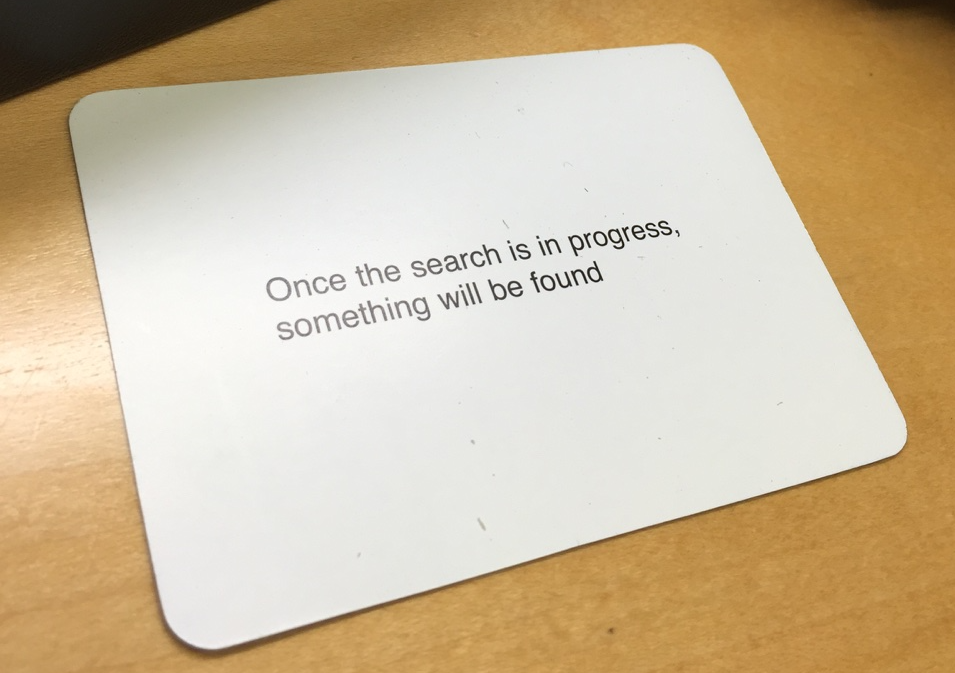
\includegraphics[width=0.5\textwidth]{figures/oblique_strategies_cropped.png}
\end{figure}



%\begin{flushright}AUSTIN PATRICK SOUSA     \end{flushright}
\noindent Austin Patrick Sousa \\
\emph{Boulder, Colorado}\\
\emph{June 1, 2018}

\vspace{20mm}

\noindent This work was supported in part by the Air Force Research Lab under contract FA9453-12-C-0217; the National Science Foundation under grants NSF-HAIL/AGS-1139321 and NSF-CEDAR/AGS-1243176; and Oswald Garrison Villard, Jr. Graduate Student Fellowship for students in radioscience.

%\hspace{0.1\textwidth} May 2018 

%\hspace{0.1\textwidth} Boulder, CO
